\documentclass[10pt]{beamer}

\usetheme[progressbar=frametitle, numbering=fraction,]{metropolis}

\usepackage{booktabs}
\usepackage{pgfplots}
\usepgfplotslibrary{dateplot}
\usepackage{texshade}      
\usepackage{amsmath}
\usepackage{amssymb}
\usepackage{xspace}
\usepackage{xcolor}
\usepackage{appendixnumberbeamer}
\usepackage{multirow}
\usepackage{verbatim}

\usepackage{tikz}
\usetikzlibrary{shapes.geometric, arrows}
\tikzstyle{startstop} = [rectangle, rounded corners, minimum width=3cm, minimum height=1cm,text centered, draw=black, fill=red!30]
\tikzstyle{io} = [trapezium, trapezium left angle=70, trapezium right angle=110, minimum width=3cm, minimum height=1cm, text centered, draw=black, fill=blue!30]
\tikzstyle{process} = [rectangle, minimum width=3cm, minimum height=1cm, text centered, draw=black, fill=orange!30]
\tikzstyle{decision} = [diamond, minimum width=3cm, minimum height=1cm, text centered, draw=black, fill=green!30]

\tikzstyle{arrow} = [thick,->,>=stealth]


\newcommand{\themename}{\textbf{\textsc{metropolis}}\xspace}

\setbeamercovered{invisible}
\setbeamertemplate{caption}{\raggedright\insertcaption\par}

\title{Grip Strength and Electromyogram(EMG)}
%\subtitle{What we see, is not what it is}
\date{\today}
\author{Saket Choudhary}
\institute{BISC 104\\Session 4}
%\titlegraphic{\hfill
\includegraphics[height=1.5cm]{logo}}

\begin{document}

\maketitle

\begin{frame}[standout]
  "\textit{Life is full of screwups. You're supposed to fail sometimes. It's a required part of the human existence.}"\\
\hfill ― Sarah Dessen, Along for the Ride
\end{frame}

\begin{frame}[fragile]{Muscle contraction strength and EMG}
\begin{itemize}[<+-| alert@+>]
\item Strength of muscle contraction is related to number of motor units activated
\item It is directly proportional to the potential generated
\item Difficult to quantify the amount of potential
\item Electromyogram(EMG) is used to measure muscular strength
\item Why Study this? EMG is used for assessing muscular health
\end{itemize}
\end{frame}

\begin{frame}[fragile]{Today's experiment}
\begin{itemize}[<+-| alert@+>]
\item \textbf{Please read the lab manual -- step by step!}
\item 3 PDFs -- Background, Setup/Calibrate, Experiment Activity
\item Step 1: \textbf{"EMG Cable and Hand Dynamometer Setup"}
\item Step 2: \textbf{"Calibrating the Hand Dynamometer"} -- \textbf{Method 2}
\item Weigh textbooks in \textbf{kilograms}. 1kg = 2.2lb
\item Step 3: Proceed to \textbf{"Experiment HM-1"}
\item Exercise 1 and 2 are compulsory.
\end{itemize}
\end{frame}

\begin{frame}[fragile]{Analysis -- Area Under Curve}
\begin{figure}
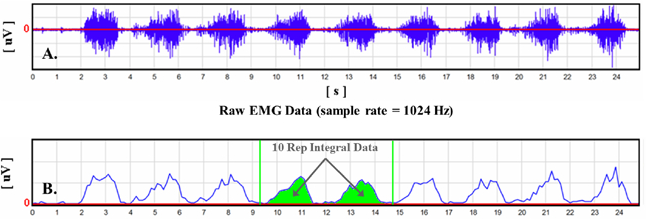
\includegraphics[width=\linewidth]{emg}
\end{figure}
\end{frame}

\begin{frame}[fragile]{Electrodes}
\begin{figure}
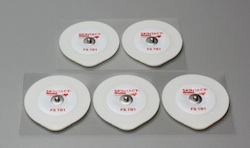
\includegraphics[width=\linewidth]{electrodes}
\end{figure}
\end{frame}

\begin{frame}[fragile]{Dynamometer}
\begin{figure}
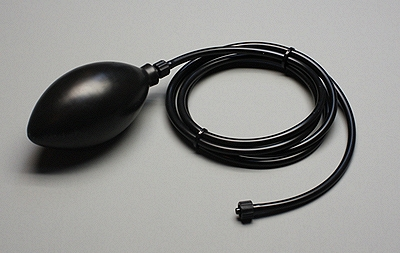
\includegraphics[width=\linewidth]{FT-220}
\end{figure}
\end{frame}



\begin{frame}[fragile]{Office Hours}
\Large \begin{center}Tuesday: 9-10AM\\
Thursday: 9-10AM\\
ZSH 372\\
\vspace*{2cm}
Saket Choudhary\\ 
skchoudh@usc.edu\\
\end{center}


\end{frame}

\end{document}
